Los LEDs se utilizan para dar una alerta visual al usuario sobre el reconocimiento de los materiales. Los LEDs están distribuidos de la siguiente manera:

\begin{itemize}
  \item \textbf{Azul:} indica que se ha reconocido plástico. Pin D3.
  \item \textbf{Verde:} indica que se ha reconocido cartón. Pin D4.
  \item \textbf{Rojo:} indica que no se ha podido reconcer nigún material. Pin D5.
\end{itemize}

Para determinar un forma adecuada de conectarlos se consideraron valores promedios obtenidos de DataSheets~\cite{led_datasheet}. En un entorno ideal  los valores serían los siguientes:

\begin{itemize}
  \item \textbf{Voltaje de la fuente $(V_s)$:} $3.3 V$. Los voltajes que entrega el ESP32S3.
  \item \textbf{Caída de voltaje típica en un LED $(V_{LED})$:} $2 V$.
  \item \textbf{Corriente óptima en un LED $(I)$:} $20 mA$.
\end{itemize}

Se aplica la Ley de Ohm y el principio de conservación de voltajes. La suma de las caídas de voltaje en el circuito debe igualar el voltaje de la fuente. Se considera la caida de voltaje en el resistor como $V_R$:

\[ V_s = V_R + V_{LED} \]

Por lo tanto, la caída de voltaje en el resistor es:

\[ V_R = V_s - V_{LED} = 3.3 V - 2 V = 1.3 V \]

Conociendo que la corriente $I$ idonea es $20 mA$, se calcula el valor óptimo del resistor:

\[ R = \frac{V_R}{I} = \frac{1.3 V}{20 mA} = 65 \Omega \]

\begin{figure}[H]
	\centering
	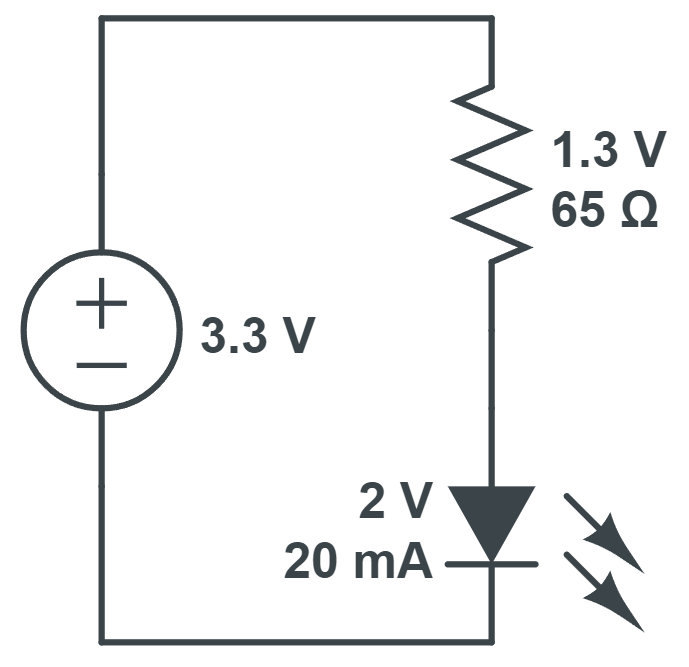
\includegraphics[scale  = 0.30]{Imagenes/led_ideal.png}
	\caption{Circuito LED ideal}{Fuente: Propia}
\end{figure}

Dado que no se cuenta con un resistor de exactamente $65 \Omega$ se optó por utilizar uno de $100 \Omega$. Por lo tanto, se realiza una operación parecida a la anterior. Se parten de los siguientes datos:

\begin{itemize}
  \item \textbf{Voltaje de la fuente $(V_s)$:} $3.3 V$. Los voltajes que entrega el ESP32S3.
  \item \textbf{Caída de voltaje típica en un LED $(V_{LED})$:} $2 V$.
  \item \textbf{Valor del resistor $(R)$:} $100 \Omega$.
\end{itemize}

La caida de voltaje en el resitor es la misma $V_R = 1.3 V$. Por consiguiente la corriente que fluye por el circuito es:

\[ I = \frac{V_R}{R} = \frac{1.3 V}{100 \Omega} = 13 mA \]

\begin{figure}[H]
	\centering
	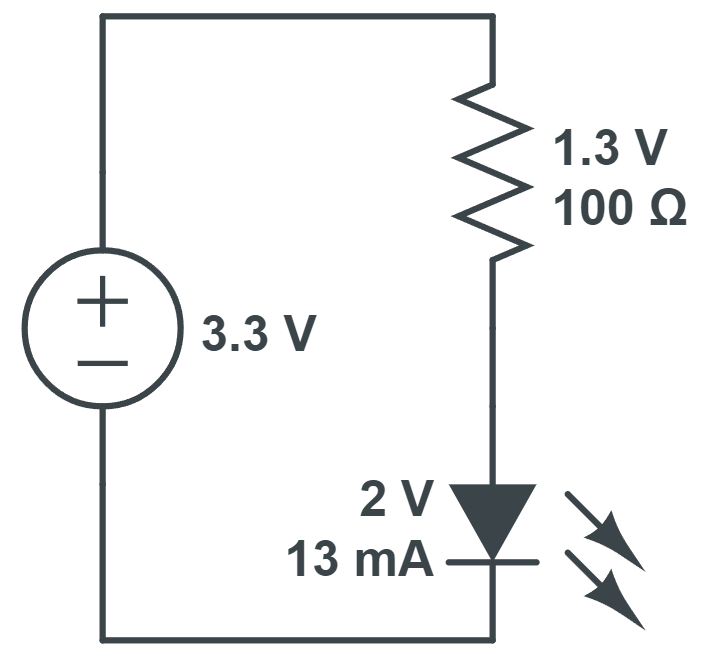
\includegraphics[scale  = 0.30]{Imagenes/led_real.png}
	\caption{Circuito LED real}{Fuente: Propia}
\end{figure}

Los LEDs brillarán por debajo de su intensidad óptima. Para calcular la caída de intensidad en términos porcentuales, se usa la fórmula de porcentaje de reducción:

\[ Caída(\%) = \frac{\text{Intensidad óptima} - \text{Intensidad actual}}{\text{Intensidad óptima}} * 100 = \frac{20 - 13}{20} * 100 = 35\% \]

La caída de intensidad es de un 35\%.